% Source: AESP_466_ClassWork/Assignments/Assignment_2/AESP466_HW2_Reference_Sp26.tex
% Description: \textbf{Turbulent Flat Plate Skin Friction Coefficient.

\documentclass[border=4pt]{standalone}
\usepackage{amsmath}
\usepackage{amssymb}
\usepackage{graphicx}
\usepackage{pgfplots}
\usepackage{tikz}
\usepackage{xcolor}
\pgfplotsset{compat=1.18}
\usetikzlibrary{arrows.meta, calc, positioning}

\definecolor{Garnet}{HTML}{73000A}
\definecolor{USC_Rose}{HTML}{CC2E40}
\definecolor{USC_Blue}{HTML}{466A9F}
\definecolor{USC_Slate}{HTML}{1F414D}
\definecolor{USC_Olive}{HTML}{65780B}
\definecolor{USC_Lime}{HTML}{CED318}
\definecolor{USC_Gold}{HTML}{A49137}
\definecolor{USC_Black90}{HTML}{565656}
\definecolor{USC_Black10}{HTML}{ECECEC}


\begin{document}
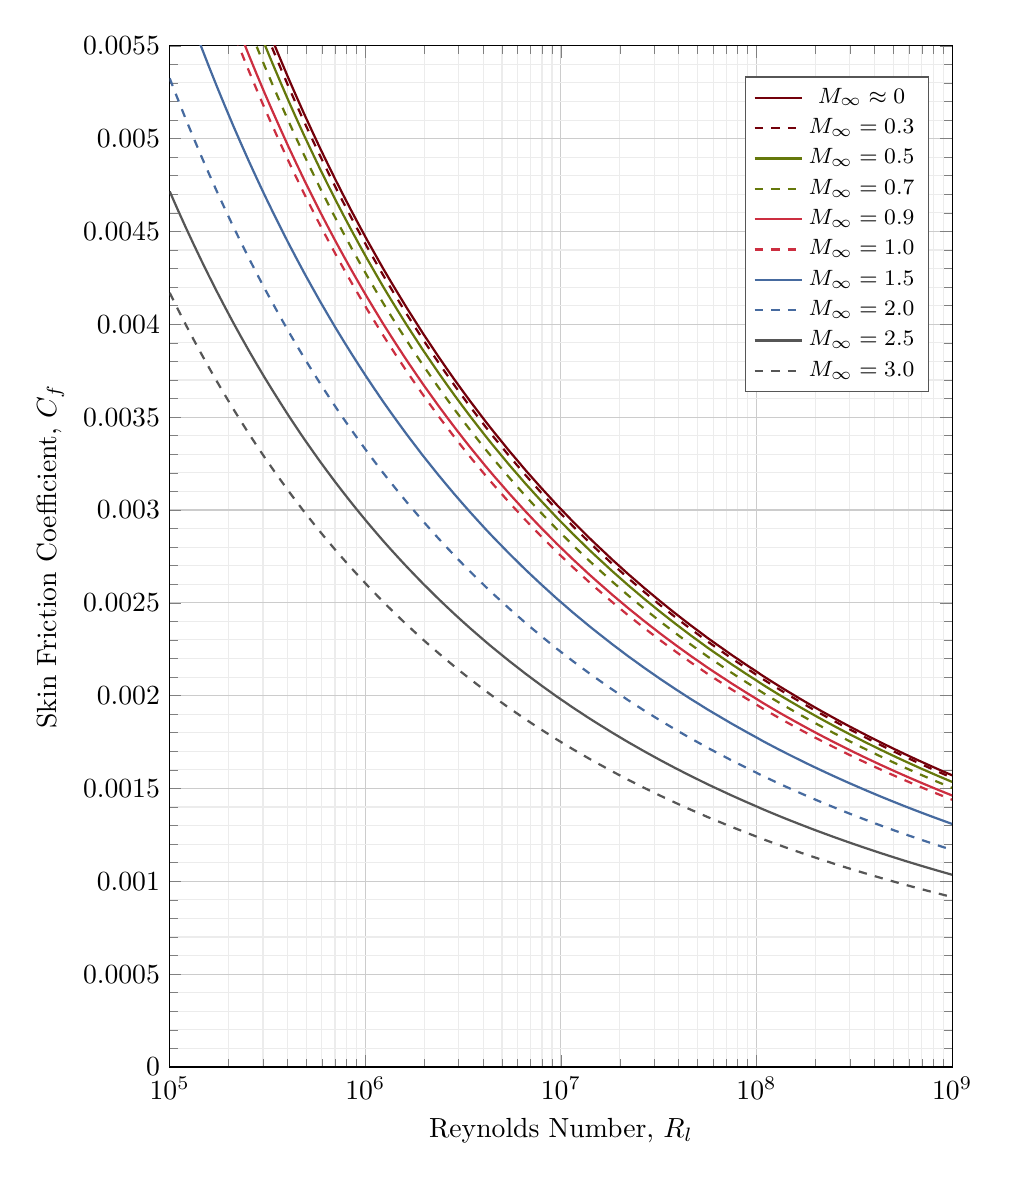
\begin{tikzpicture}
\begin{semilogxaxis}[
    width=0.95\textwidth,
    height=1.2\textwidth,
    xlabel={Reynolds Number, $R_l$},
    ylabel={Skin Friction Coefficient, $C_f$},
    grid=both,
    minor grid style={USC_Black10},
    major grid style={USC_Black90!30},
    xmin=1e5, xmax=1e9,
    ymin=0, ymax=0.0055,
    ytick distance=0.0005,
    minor y tick num=4,
    domain=1e5:1e9,
    samples=100,
    legend pos=north east,
    legend style={draw=USC_Black90, fill=white, font=\footnotesize},
    title style={font=\bfseries},
    scaled y ticks=false,
    yticklabel style={/pgf/number format/fixed, /pgf/number format/precision=4}
]

% Color scheme: Garnet (0, 0.3), Green (0.5, 0.7), Pink (0.9, 1.0), Blue (1.5, 2.0), Gray (2.5, 3.0)
% Alternating solid/dashed within each pair

% M=0 - Garnet (solid)
\addplot[thick, Garnet] {0.455 / (log10(x))^2.58};
\addlegendentry{$M_\infty \approx 0$}

% M=0.3 - Garnet (dashed)
\addplot[thick, Garnet, dashed] {0.455 / (log10(x))^2.58 / (1 + 0.144*0.3^2)^0.65};
\addlegendentry{$M_\infty = 0.3$}

% M=0.5 - Green (solid)
\addplot[thick, USC_Olive] {0.455 / (log10(x))^2.58 / (1 + 0.144*0.5^2)^0.65};
\addlegendentry{$M_\infty = 0.5$}

% M=0.7 - Green (dashed)
\addplot[thick, USC_Olive, dashed] {0.455 / (log10(x))^2.58 / (1 + 0.144*0.7^2)^0.65};
\addlegendentry{$M_\infty = 0.7$}

% M=0.9 - Pink (solid)
\addplot[thick, USC_Rose] {0.455 / (log10(x))^2.58 / (1 + 0.144*0.9^2)^0.65};
\addlegendentry{$M_\infty = 0.9$}

% M=1.0 - Pink (dashed)
\addplot[thick, USC_Rose, dashed] {0.455 / (log10(x))^2.58 / (1 + 0.144*1.0^2)^0.65};
\addlegendentry{$M_\infty = 1.0$}

% M=1.5 - Blue (solid)
\addplot[thick, USC_Blue] {0.455 / (log10(x))^2.58 / (1 + 0.144*1.5^2)^0.65};
\addlegendentry{$M_\infty = 1.5$}

% M=2.0 - Blue (dashed)
\addplot[thick, USC_Blue, dashed] {0.455 / (log10(x))^2.58 / (1 + 0.144*2.0^2)^0.65};
\addlegendentry{$M_\infty = 2.0$}

% M=2.5 - Gray (solid)
\addplot[thick, USC_Black90] {0.455 / (log10(x))^2.58 / (1 + 0.144*2.5^2)^0.65};
\addlegendentry{$M_\infty = 2.5$}

% M=3.0 - Gray (dashed)
\addplot[thick, USC_Black90, dashed] {0.455 / (log10(x))^2.58 / (1 + 0.144*3.0^2)^0.65};
\addlegendentry{$M_\infty = 3.0$}

\end{semilogxaxis}
\end{tikzpicture}
\end{document}
